\documentclass[tikz,border=10pt]{standalone}
\usetikzlibrary{calc}
\begin{document}
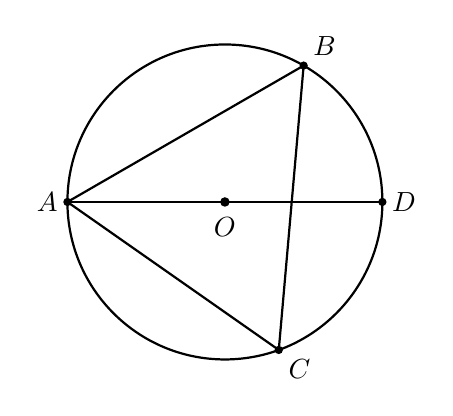
\begin{tikzpicture}    
% --- 参数定义 ---    
\def\r{2} % 设置圆的半径        
% --- 绘制圆 ---    
\draw[thick] (0,0) circle (\r);    
\filldraw (0,0) circle (1.5pt) node[below=2pt] {$O$}; % 圆心 O        
% --- 定义关键点 ---    
\coordinate (A) at (-\r, 0);    
\coordinate (D) at (\r, 0);    
% 使用极坐标定义 B 和 C (根据目测位置设定角度)    
\coordinate (B) at (60:\r);    
\coordinate (C) at (-70:\r);        
% --- 绘制线段 ---    
\draw[thick] (A) -- (D);        % 直径 AD    
\draw[thick] (A) -- (B) -- (C) -- cycle; % 三角形 ABC        
% --- 标注点 ---    
\node[left] at (A) {$A$};    
\node[right] at (D) {$D$};    
\node[above right] at (B) {$B$};    
\node[below right] at (C) {$C$};        
% --- 标记点 (可选: 补充点状效果) ---    
\fill (A) circle (1.5pt);    
\fill (D) circle (1.5pt);    
\fill (B) circle (1.5pt);    
\fill (C) circle (1.5pt);    
\end{tikzpicture}
\end{document}